\documentclass{article}
\usepackage{graphicx}
\usepackage[english]{babel}
\usepackage{tabularx,booktabs,ragged2e}
\usepackage{indentfirst}
\usepackage{listings}
\usepackage{upquote}
\usepackage{amsmath}


\newcolumntype{L}{>{\RaggedRight\arraybackslash}X}
\title{Employment and GDP}
\author{HSIU-HSUAN, YEH}


\begin{document}
\pagestyle{headings}	
\maketitle
\noindent\rule{12cm}{0.5pt}
\begin{abstract}
    In economics, there is a simple, empirical-observed relation which states 
    that the increase
    in aggregate output will lead to the decline in unemployment rate. In this 
    research, I take advantage of the statistics of employment and GDP in the 
    state level to find out whether the rule exists or not. And the main finding
    is that only those state with high employment or GDP growth rate support this
    hypothesis.
\end{abstract}
\noindent\rule{12cm}{0.5pt}
\section{Introduction}
Okun's law or Okun's rule of thumb is an empirical conclusion rather than the
theoretical results. In original statements by Arthur Melvin Oken in 1962, a
 2\% increase in output corresponds to 1 \% decline in the rate
of cyclical unemployment. And the intuition is straight-forward: the increase in 
output will need more labor force. Although the rule seems to be reasonable, 
it can not be observed everywhere, for example, China
has different situation since the unemployment is only counted within city.
In the following section, I will pick 4 states which the employment or GDP growth
rate are either highest or lowest to see whether the rule exists or not. The 4 states are West Virginia, Utah, Louisiana
and North Dakota. West Virginia has the lowest average employment growth rate while
Utah has the highest from 1997 to 2021. In another aspect, Louisiana has the 
lowest average GDP growth rate while North Dakota has the highest from 1997 to 
2021. The reason to check both the highest and lowest GDP and employment growth
rate is that the Okun's rule seems to only exist in high GDP or employment growth rate which
can be observed in the figure in the reference section.


\begin{center}
\begin{tabular}{lcccccc} \hline
    & (1) & (2) & (3) \\
    VARIABLES & lag\_corr & lag\_corr & lag\_corr \\ \hline
     &  &  &  \\
    emp\_gr & 0.148*** &  & 0.0889 \\
     & (0.0312) &  & (0.0581) \\
    gdp\_gr &  & 0.104*** & 0.0556 \\
     &  & (0.0277) & (0.0491) \\
    Constant & 0.0650 & 0.00650 & 0.0135 \\
     & (0.0443) & (0.0616) & (0.0671) \\
     &  &  &  \\
    Observations & 60 & 60 & 60 \\
     R-squared & 0.205 & 0.198 & 0.229 \\ \hline
    \multicolumn{4}{c}{ Robust standard errors in parentheses} \\
\end{tabular}
\end{center}

After Perform simple linear regression and the samples are the states in U.S.A,
we can observe that if a state's employment rate increase by 1\% the correlation 
coefficient between employment growth rate and lag 1 period GDP growth rate will
increase 0.148. Condition is much alike in terms of real GDP growth rate. Since
the employment growth rate and real GDP growth rate is highly correlated, coefficients
in regression are not significant. My interpretation of this phenomenon is that
maybe the states with high GDP growth rate or employment growth rate are those
in developed and thus the industries of the state are more labor-intensive. And
it makes sense that the employment of a state where the industries are labor-intensive
is highly correlated with its GDP.

\section{Case Study}
\subsection{minimum average employment growth rate: West Virginia}
\begin{figure}[h]
	\centering
	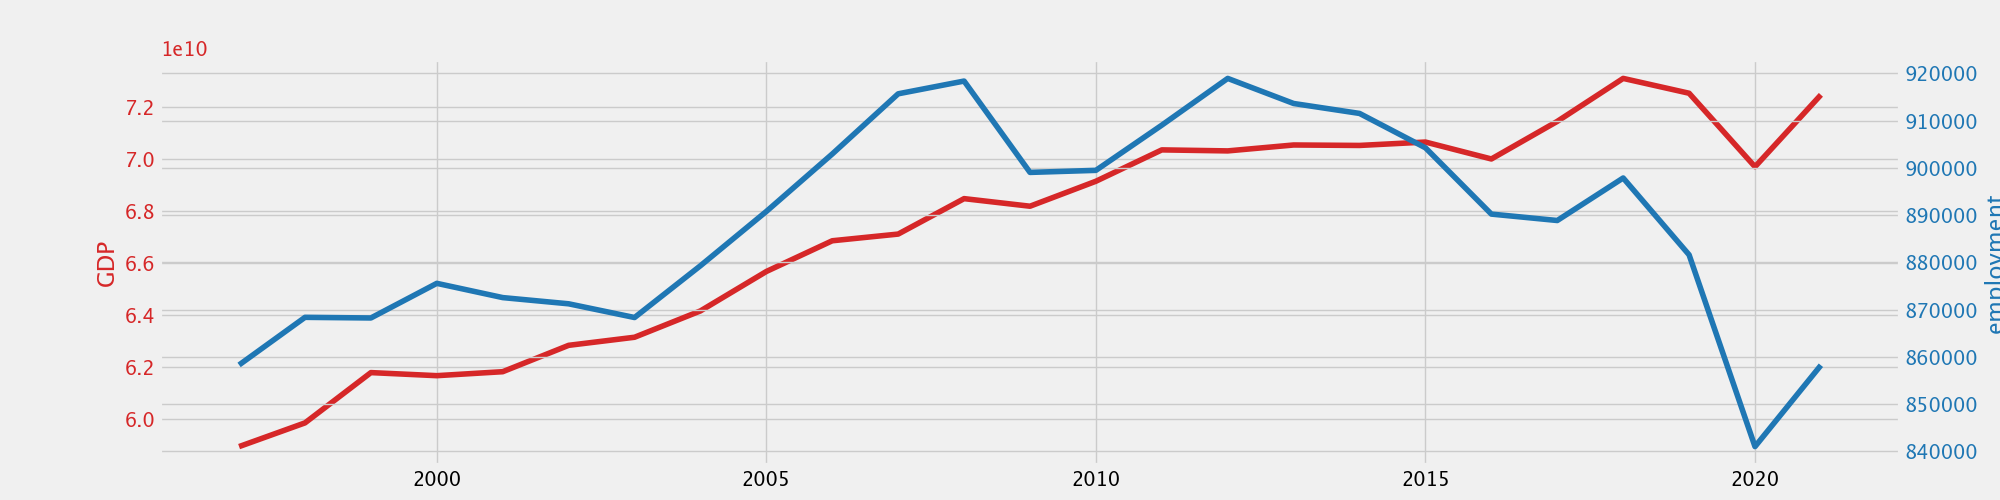
\includegraphics[width=12cm, height=4cm]{res/wv.png}
	\caption{Real GDP and Employment of West Virginia}
\end{figure}


\begin{center}
\resizebox{10cm}{!}
{
\begin{tabular}{lccccc} \hline
    & (1) & (2) & (3) & (4) & (5) \\
    VARIABLES & emp\_gr & emp\_gr & emp\_gr & emp\_gr & emp\_gr \\ \hline
    &  &  &  &  &  \\
    L.gdp\_gr & 0.0776 &  &  &  &  \\
    & (0.212) &  &  &  &  \\
    L.emp\_gr &  & 0.0806 & 0.264 &  & 0.362 \\
    &  & (0.224) & (0.246) &  & (0.263) \\
    L2.emp\_gr &  &  & -0.584* & -0.433 & -0.774** \\
    &  &  & (0.333) & (0.303) & (0.365) \\
    L3.emp\_gr &  &  &  &  & 0.313 \\
    &  &  &  &  & (0.360) \\
    Constant & -0.0982 & -0.0342 & 0.0684 & 0.0135 & -0.0414 \\
    & (0.352) & (0.315) & (0.320) & (0.317) & (0.331) \\
    &  &  &  &  &  \\
    Observations & 23 & 23 & 22 & 22 & 21 \\
    R-squared & 0.006 & 0.006 & 0.145 & 0.093 & 0.215 \\ \hline
    \multicolumn{6}{c}{ Standard errors in parentheses} \\
\end{tabular}
}
\end{center}

\vspace{0.4cm}

\subsection{minimum average GDP growth rate: Louisiana}
\begin{center}
\resizebox{10cm}{!}
{
    \begin{tabular}{lccccc} \hline
        & (1) & (2) & (3) & (4) & (5) \\
       VARIABLES & emp\_gr & emp\_gr & emp\_gr & emp\_gr & emp\_gr \\ \hline
        &  &  &  &  &  \\
       L.gdp\_gr & -0.110 &  &  &  &  \\
        & (0.0955) &  &  &  &  \\
       L.emp\_gr &  & 0.0491 &  & 0.168 & 0.272 \\
        &  & (0.217) &  & (0.215) & (0.240) \\
       L2.emp\_gr &  &  & -0.605* & -0.667** & -0.849** \\
        &  &  & (0.292) & (0.305) & (0.326) \\
       L3.emp\_gr &  &  &  &  & 0.291 \\
        &  &  &  &  & (0.340) \\
       Constant & 0.598* & 0.515 & 1.012** & 0.979** & 0.733 \\
        & (0.322) & (0.350) & (0.388) & (0.394) & (0.474) \\
        &  &  &  &  &  \\
       Observations & 23 & 23 & 22 & 22 & 21 \\
        R-squared & 0.060 & 0.002 & 0.177 & 0.202 & 0.287 \\ \hline
       \multicolumn{6}{c}{ Standard errors in parentheses} \\
       \multicolumn{6}{c}{ *** p$<$0.01, ** p$<$0.05, * p$<$0.1} \\
\end{tabular}
}
\end{center}

In the above two states, West Virginia and Louisiana the lag 1 GDP explanatory
variable is not significant and the most explanatory variable is the lag 2 
employment. However, In the next two states, Utah and North Dakota the lag 1 GDP
explanatory variable is the most explanatory and also significant. Notice that
the Utah has the highest average employment growth rate and North Dakota has the 
highest average GDP growth rate.So I conclude that the Oken's rule of thumb only
holds within those states with high average employment or GDP growth rate. For more
information(stationary, q test) check the reference.

\newpage

\subsection{maximum average employment growth rate: Utah}
\begin{figure}[h]
	\centering
	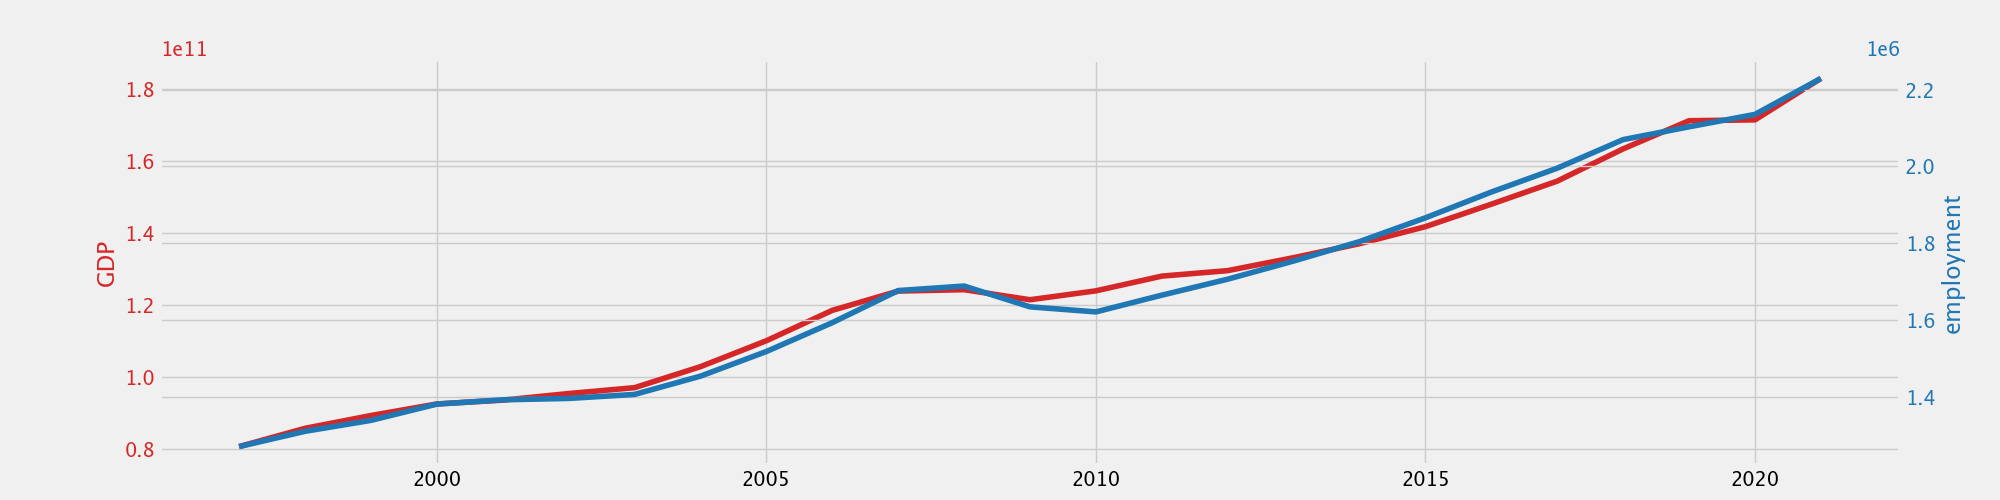
\includegraphics[width=12cm, height=3cm]{res/ut.png}
	\caption{Real GDP and Employment of Utah}
\end{figure}

\begin{center}
\resizebox{9cm}{!}
{
    \begin{tabular}{lccccc} \hline
    & (1) & (2) & (3) & (4) & (5) \\
    VARIABLES & emp\_gr & emp\_gr & emp\_gr & emp\_gr & emp\_gr \\ \hline
    &  &  &  &  &  \\
    L.gdp\_gr & 0.439*** & 0.576*** & 0.579*** & 0.451*** & 0.392* \\
    & (0.151) & (0.155) & (0.181) & (0.144) & (0.194) \\
    L2.emp\_gr &  & -0.371* &  &  &  \\
    &  & (0.187) &  &  &  \\
    L2.gdp\_gr &  &  & -0.206 &  & 0.115 \\
    &  &  & (0.182) &  & (0.244) \\
    L3.gdp\_gr &  &  &  & -0.358** & -0.425* \\
    &  &  &  & (0.146) & (0.206) \\
    Constant & 0.885 & 1.377** & 1.221 & 2.125** & 2.156** \\
    & (0.620) & (0.646) & (0.711) & (0.781) & (0.801) \\
    &  &  &  &  &  \\
    Observations & 23 & 22 & 22 & 21 & 21 \\
    R-squared & 0.286 & 0.431 & 0.357 & 0.483 & 0.489 \\ \hline
    \multicolumn{6}{c}{ Standard errors in parentheses} \\
\end{tabular}
}
\end{center}

\subsection{maximum average employment growth rate: North Dakota}
\begin{center}
\resizebox{9cm}{!}
{
\begin{tabular}{lccccc} \hline
        & (1) & (2) & (3) & (4) & (5) \\
       VARIABLES & emp\_gr & emp\_gr & emp\_gr & emp\_gr & emp\_gr \\ \hline
        &  &  &  &  &  \\
       L.gdp\_gr & 0.213** & 0.231** & 0.199** & 0.230** & 0.212** \\
        & (0.0814) & (0.0927) & (0.0870) & (0.0891) & (0.0927) \\
       L2.emp\_gr &  & -0.0895 &  &  &  \\
        &  & (0.239) &  &  &  \\
       L2.gdp\_gr &  &  & 0.0673 &  & 0.0781 \\
        &  &  & (0.0902) &  & (0.0962) \\
       L3.gdp\_gr &  &  &  & -0.0498 & -0.0651 \\
        &  &  &  & (0.0925) & (0.0953) \\
       Constant & 0.311 & 0.429 & 0.134 & 0.498 & 0.305 \\
        & (0.559) & (0.613) & (0.653) & (0.708) & (0.753) \\
        &  &  &  &  &  \\
       Observations & 23 & 22 & 22 & 21 & 21 \\
        R-squared & 0.246 & 0.260 & 0.276 & 0.270 & 0.298 \\ \hline
       \multicolumn{6}{c}{ Standard errors in parentheses} \\
       \multicolumn{6}{c}{ *** p$<$0.01, ** p$<$0.05, * p$<$0.1} \\
\end{tabular}
}
\end{center}



\newpage
\section{Reference}
\subsection{more plots}
\begin{figure}[h]
	\centering
	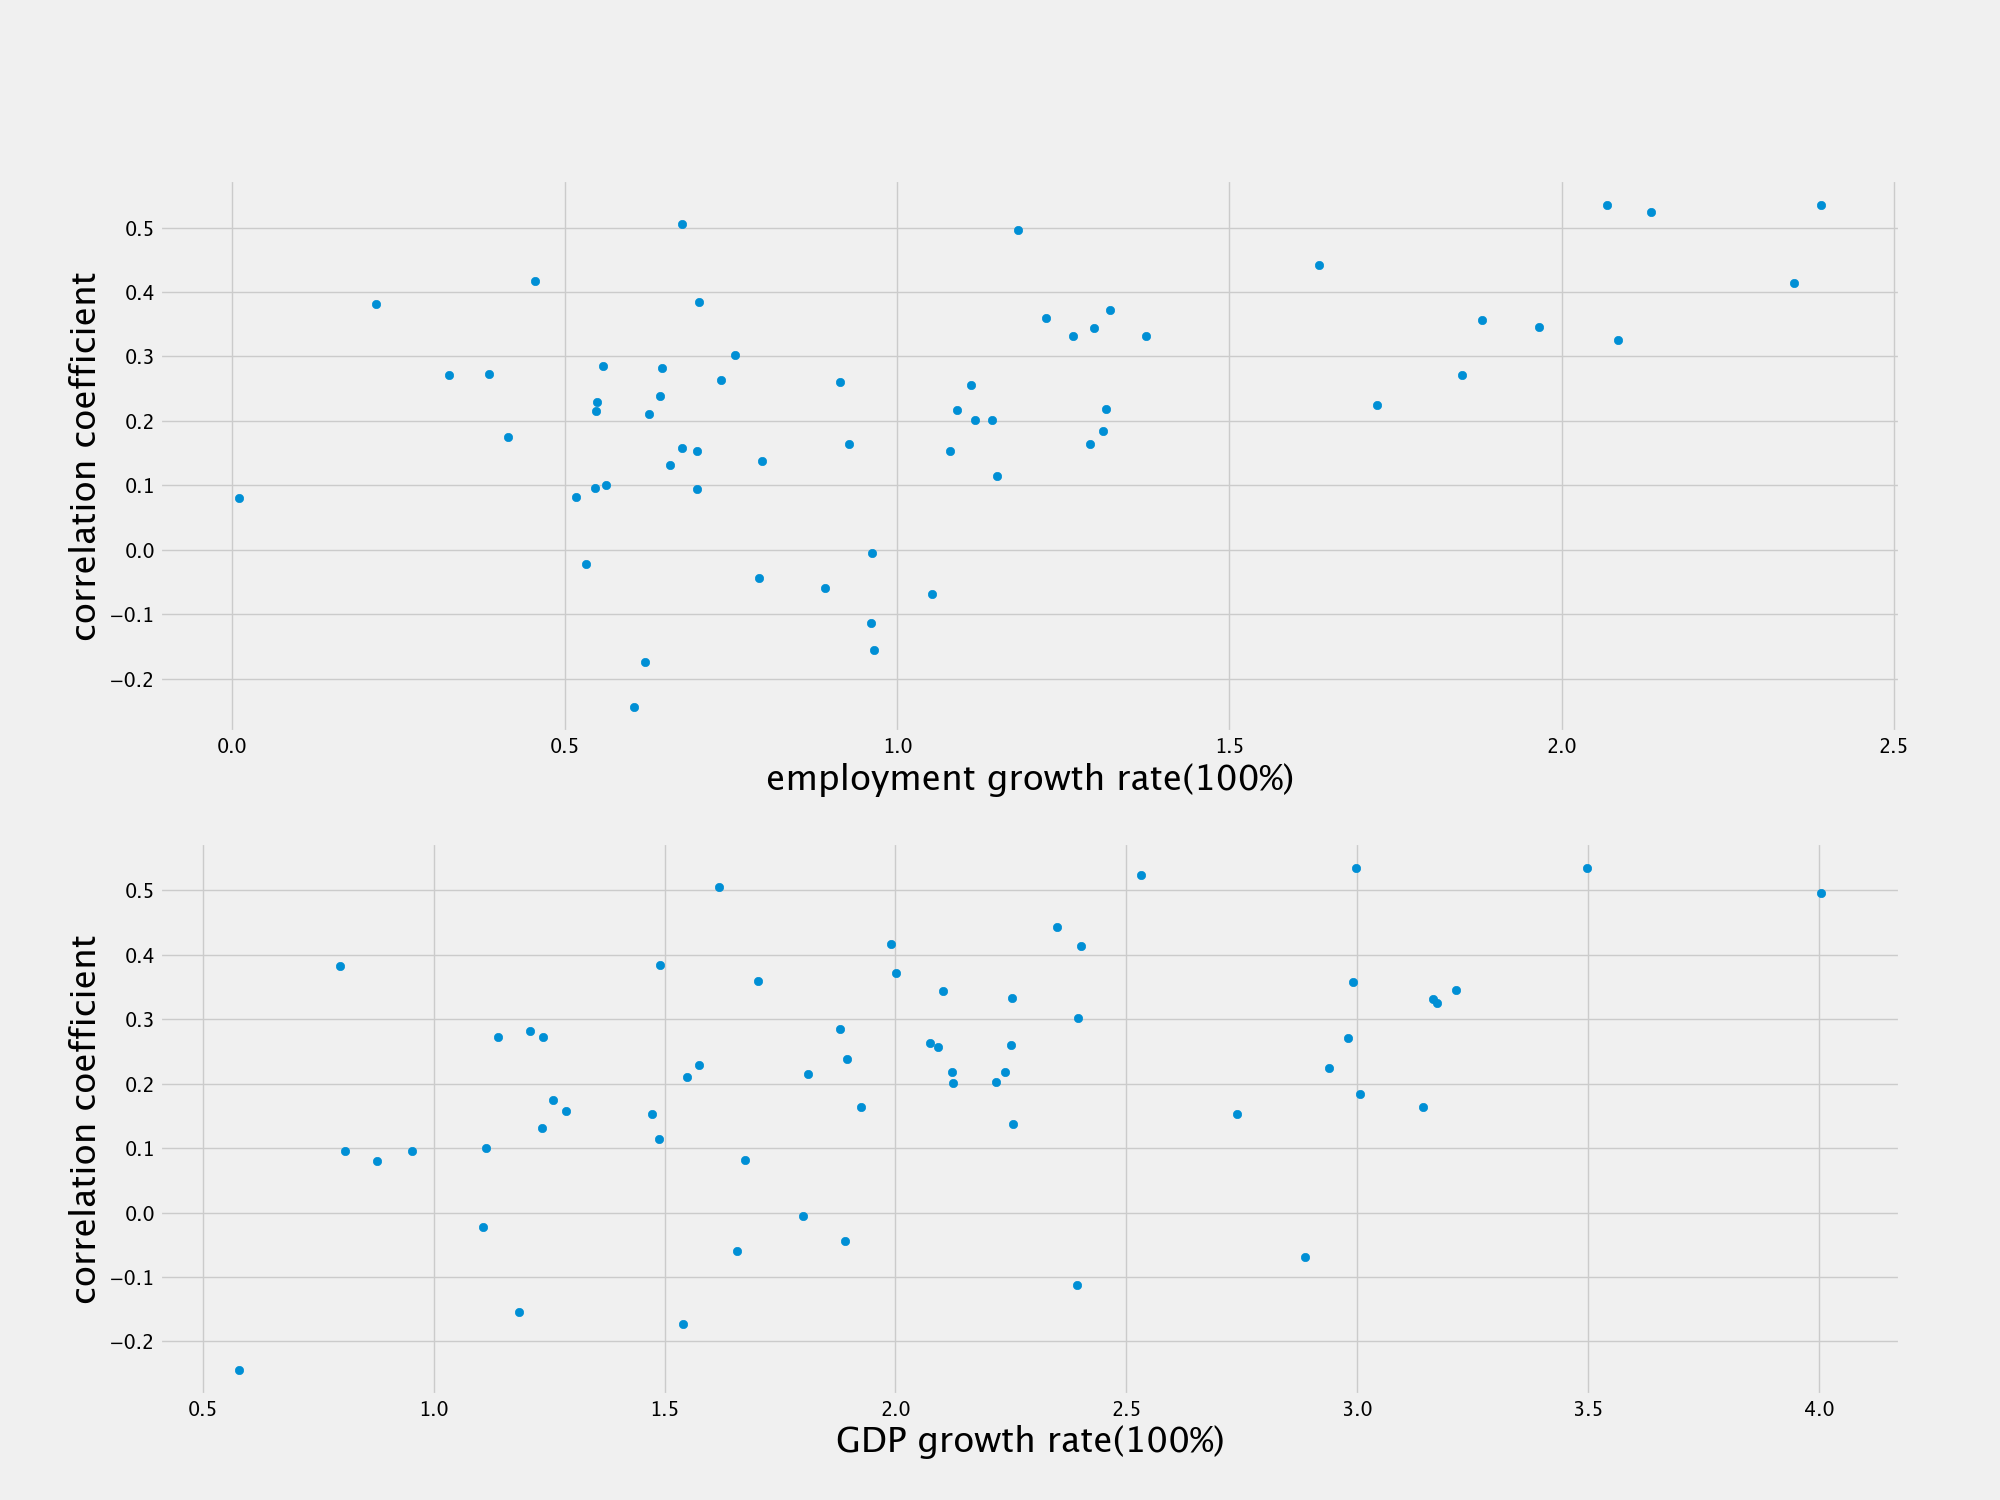
\includegraphics[width=12cm, height=5cm]{res/corr.png}
	\caption{
        Correlation coefficient between employment growth rate and lag 1 period GDP growth rate
        versus employment and real GDP growth rate
    }
\end{figure}

\begin{figure}[h]
	\centering
	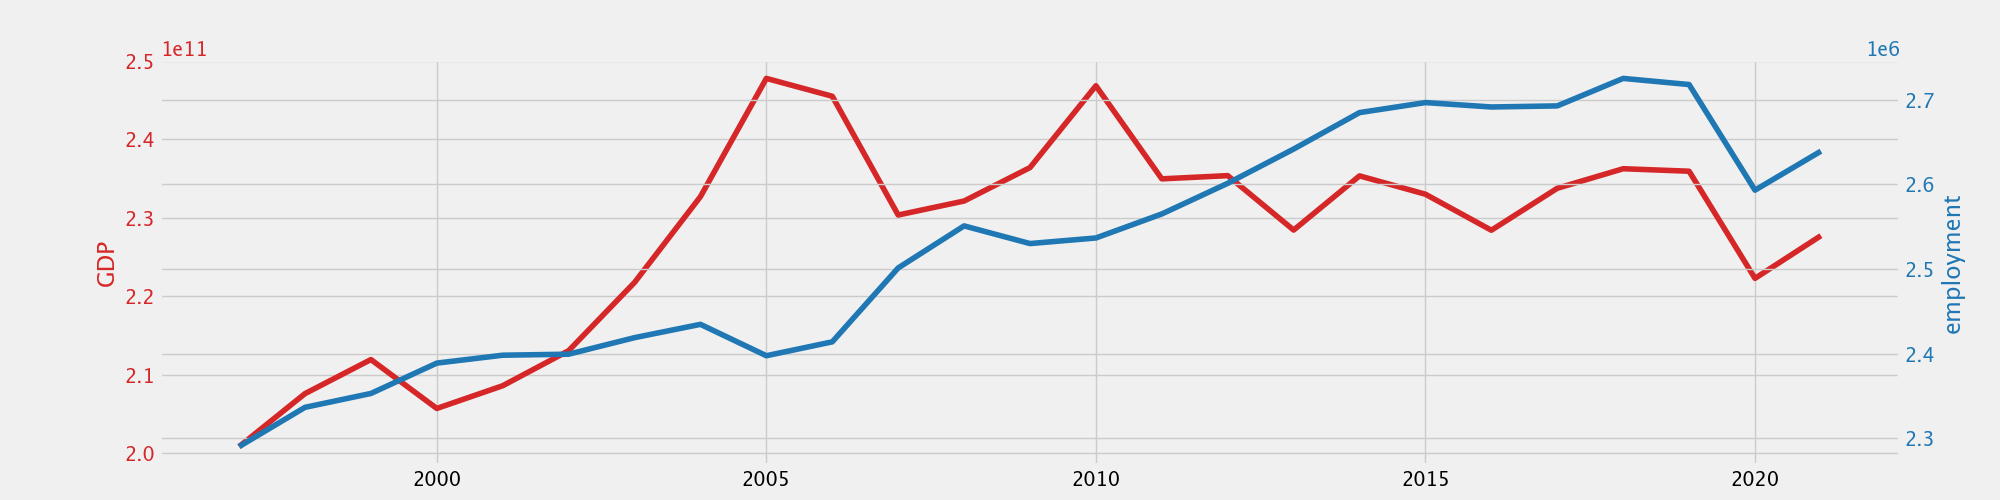
\includegraphics[width=12cm, height=2.5cm]{res/la.png}
	\caption{Real GDP and Employment of Louisiana}
\end{figure}

\begin{figure}[h]
	\centering
	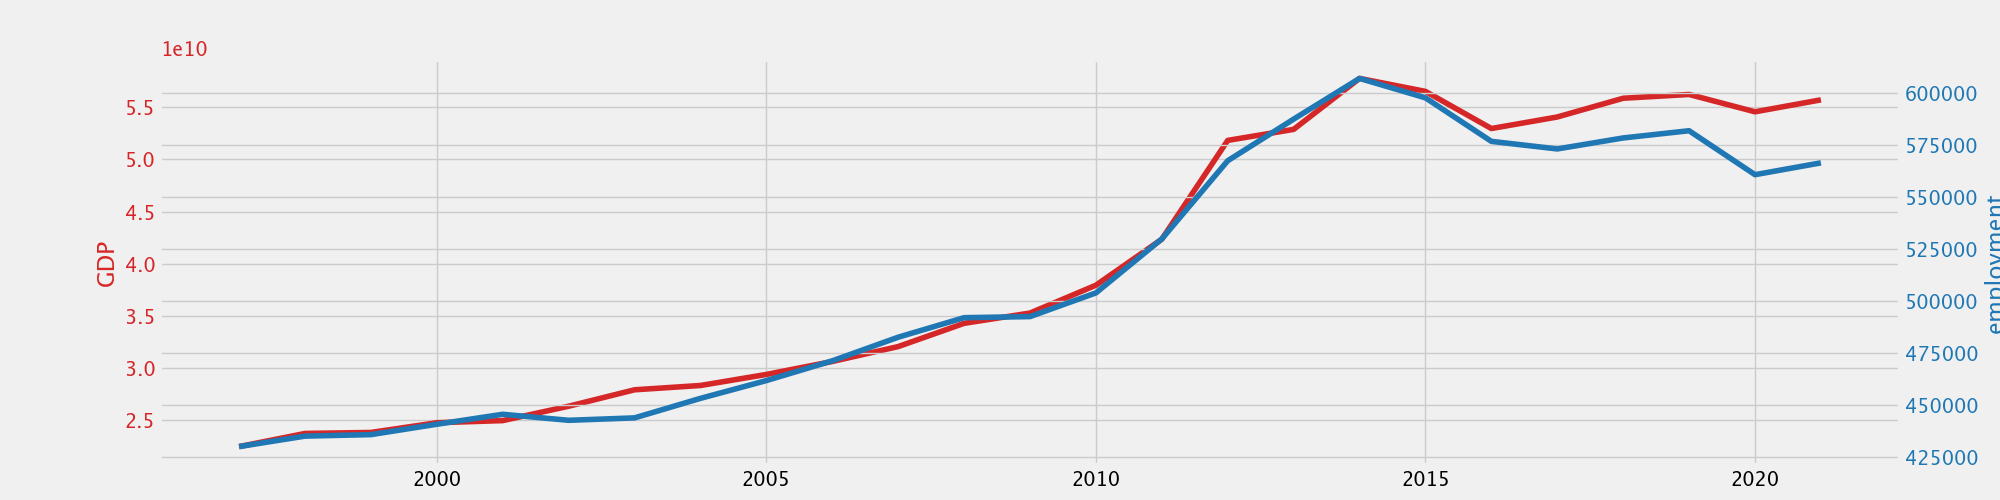
\includegraphics[width=12cm, height=2.5cm]{res/nd.png}
	\caption{Real GDP and Employment of North Dakota}
\end{figure}

\newpage

\subsection{Stationary Test}
\vspace{0.5cm}
\subsubsection{West Virginia}
\noindent \textbf{ADF test for employment growth rate: }
\begin{center}
    \resizebox{13cm}{!}
    {
    \begin{tabular}{lcccccc} \hline
        Test Statistics & 1\% Critical Value& 5\% Critical Value & 10\% Critical Value \\ \hline
        -4.096 & -3.750 & -3.0 & -2.63 \\ \hline
    \end{tabular}
    }
\end{center}

\vspace{0.5cm}

\noindent \textbf{DF-GLS test for employment growth rate with no trend, max lag=3:}
\begin{center}
\resizebox{13cm}{!}
{
\begin{tabular}{lcccccc} \hline
    [lags] & mu Test Statistics & 1\% Critical Value& 5\% Critical Value & 10\% Critical Value \\ \hline
    3      & -1.268 & -2.660 & -2.396 & -2.055 \\ 
    2      & -1.773 & -2.660 & -2.462 & -2.121 \\
    1      & -3.739 & -2.660 & -2.528 & -2.183 \\ \hline
\end{tabular}
}
\end{center}

\vspace{0.5cm}

\noindent \textbf{ADF test for employment growth rate with lag 1 period: }
\begin{center}
\resizebox{13cm}{!}
{
\begin{tabular}{lcccccc} \hline
    Test Statistics & 1\% Critical Value& 5\% Critical Value & 10\% Critical Value \\ \hline
    -4.125 & -3.750 & -3.0 & -2.63 \\ \hline
\end{tabular}
}
\end{center}

\vspace{0.5cm}

\subsubsection{Louisiana}
\noindent \textbf{ADF test for employment growth rate: }
\begin{center}
    \resizebox{13cm}{!}
    {
    \begin{tabular}{lcccccc} \hline
        Test Statistics & 1\% Critical Value& 5\% Critical Value & 10\% Critical Value \\ \hline
        -4.391 & -3.750 & -3.0 & -2.63 \\ \hline
    \end{tabular}
    }
\end{center}

\vspace{0.5cm}

\noindent \textbf{DF-GLS test for employment growth rate with no trend, max lag=5:}
\begin{center}
\resizebox{13cm}{!}
{
\begin{tabular}{lcccccc} \hline
    [lags] & mu Test Statistics & 1\% Critical Value& 5\% Critical Value & 10\% Critical Value \\ \hline
    3      & -1.744 & -2.660 & -2.396 & -2.055 \\ 
    2      & -1.843 & -2.660 & -2.462 & -2.121 \\
    1      & -4.113 & -2.660 & -2.528 & -2.183 \\ \hline
\end{tabular}
}
\end{center}

\vspace{0.5cm}

\noindent \textbf{ADF test for employment growth rate with lag 1 period: }
\begin{center}
\resizebox{13cm}{!}
{
\begin{tabular}{lcccccc} \hline
    Test Statistics & 1\% Critical Value& 5\% Critical Value & 10\% Critical Value \\ \hline
    -4.613 & -3.750 & -3.0 & -2.63 \\ \hline
\end{tabular}
}
\end{center}

\vspace{0.5cm}

\subsubsection{Utah}
\noindent \textbf{ADF test for employment growth rate: }
\begin{center}
    \resizebox{13cm}{!}
    {
    \begin{tabular}{lcccccc} \hline
        Test Statistics & 1\% Critical Value& 5\% Critical Value & 10\% Critical Value \\ \hline
        -2.535 & -3.750 & -3.0 & -2.63 \\ \hline
    \end{tabular}
    }
\end{center}

\vspace{0.5cm}

\noindent \textbf{DF-GLS test for employment growth rate with no trend, max lag=5:}
\begin{center}
\resizebox{13cm}{!}
{
\begin{tabular}{lcccccc} \hline
    [lags] & mu Test Statistics & 1\% Critical Value& 5\% Critical Value & 10\% Critical Value \\ \hline
    5      & -1.976 & -3.770 & -2.947 & -2.555 \\
    4      & -2.580 & -3.770 & -3.052 & -2.678 \\
    3      & -3.319 & -3.770 & -3.194 & -2.824 \\
    3      & -2.629 & -3.770 & -3.347 & -2.972 \\
    1      & -4.180 & -3.770 & -3.485 & -3.10 \\ \hline
\end{tabular}
}
\end{center}

\vspace{0.5cm}

\noindent \textbf{ADF test for employment growth rate with lag 3 period: }
\begin{center}
\resizebox{13cm}{!}
{
\begin{tabular}{lcccccc} \hline
    Test Statistics & 1\% Critical Value& 5\% Critical Value & 10\% Critical Value \\ \hline
    -2.964 & -3.750 & -3.0 & -2.63 \\ \hline
\end{tabular}
}
\end{center}

\vspace{0.5cm}


\subsubsection{North Dakota}
\noindent \textbf{ADF test for employment growth rate: }
\begin{center}
    \resizebox{13cm}{!}
    {
    \begin{tabular}{lcccccc} \hline
        Test Statistics & 1\% Critical Value& 5\% Critical Value & 10\% Critical Value \\ \hline
        -2.528 & -3.750 & -3.0 & -2.63 \\ \hline
    \end{tabular}
    }
\end{center}

\vspace{0.5cm}

\noindent \textbf{DF-GLS test for employment growth rate with no trend, max lag=5:}
\begin{center}
\resizebox{13cm}{!}
{
\begin{tabular}{lcccccc} \hline
    [lags] & mu Test Statistics & 1\% Critical Value& 5\% Critical Value & 10\% Critical Value \\ \hline
    3      & -1.843 & -2.660 & -2.396 & -2.055 \\ 
    2      & -2.213 & -2.660 & -2.462 & -2.121 \\
    1      & -2.632 & -2.660 & -2.528 & -2.183 \\ \hline
\end{tabular}
}
\end{center}

\vspace{0.5cm}

\noindent \textbf{ADF test for employment growth rate with lag 1 period: }
\begin{center}
\resizebox{13cm}{!}
{
\begin{tabular}{lcccccc} \hline
    Test Statistics & 1\% Critical Value& 5\% Critical Value & 10\% Critical Value \\ \hline
    -2.721 & -3.750 & -3.0 & -2.63 \\ \hline
\end{tabular}
}
\end{center}

\newpage

\subsection{White noise test}
\noindent \textbf{Portmanteau (Q) test for white noise} \\
\textit{null hypothesis: the residual is white noise} \\ 
\textit{note: all the models are chosen from the last result, ex: select AR(3) for Louisiana}
\begin{center}
\begin{tabular}{lcccccc} \hline
        state & p-value \\ \hline
        West Virginia &  0.9944 \\ 
        Louisiana &  0.9987 \\
        Utah &  0.6861 \\
        North Dakota &  0.3735 \\ \hline
 \end{tabular}
\end{center}



\end{document}